\section{Index Construction}
\label{preprocessing}

This section describes our index construction algorithm. Previous works have studied various landmark selection strategies which have a significant impact on the accuracy of online query. In our study, we observe that even with the same landmark set, choosing which shortest path from vertex to landmark to be indexed also plays an important role for the accuracy of online search. 

\begin{figure*}[ht]
    \centering
    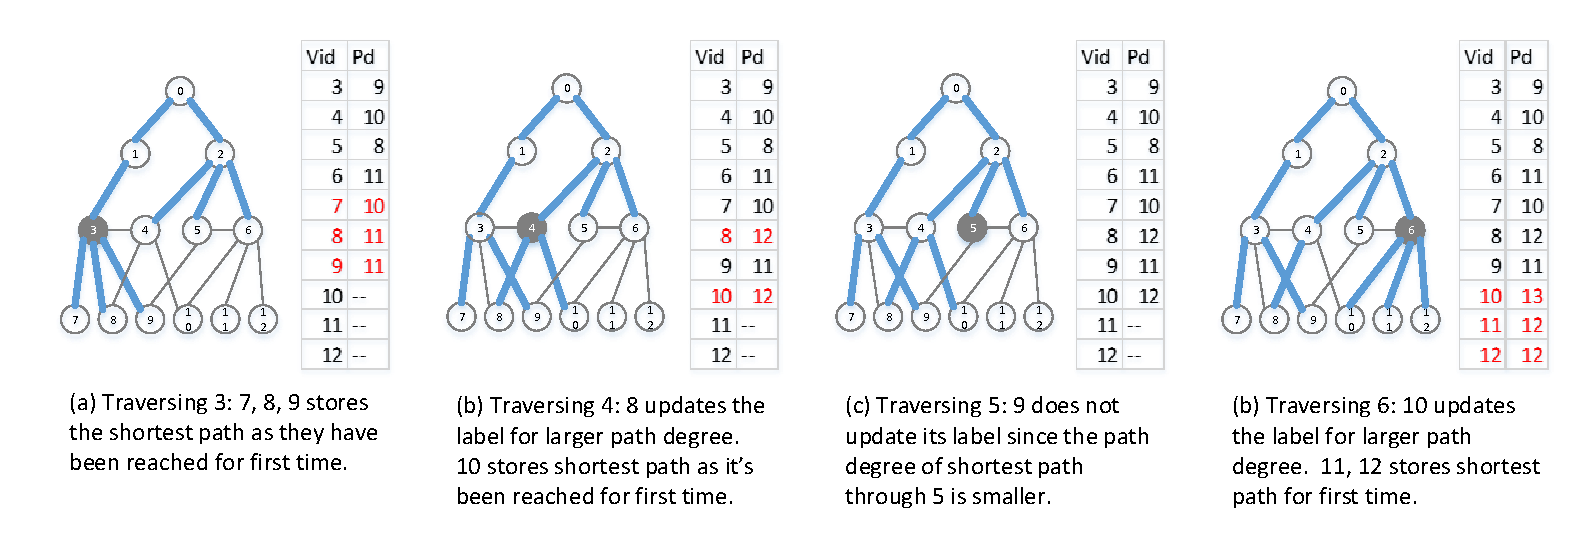
\includegraphics[width=\linewidth]{./figures/new_illustrate/bfs_illustrate.pdf}
    \caption{Greedy algorithm that index shortest path with highest path degree during breadth first search}
    \label{fig:bfs_illustrate}
\end{figure*}

\subsection{Greedy index construction algorithm}
\begin{algorithm}
    \caption{Algorithm greedy index construction vertex program running on $u$}
		\label{alg:ind}
    \begin{algorithmic}
				\Function{Index construction}{$root$}
					\State $PD \gets \emptyset$
					\State $L \gets \emptyset$
					\State $Q \gets \emptyset$
					\State $L[root.id] = root.id$
					\State $PD[root.id] = root.degree$
					\State $Q.push(root)$
					\While{$Q \neq \emptyset$}
						\State $u = Q.pop()$
						\For{$each v adjecent to u$}
							\If{$v.id \not \in L$}
								\State $L[v.id] = L[u.id] \cup v.id$
								\State $PD[v.id] = PD[u.id] + u.degree$
								\State $Q.push(v)$
							\ElsIf{$L(v).size() < L(u).size() + 1$}
								\State $continue$
							\ElsIf{PD[v.id] < PD[u.id] + u.degree}
								\State $L[v.id] = L[u.id] \cup v.id$
								\State $PD[v.id] = PD[u.id] + u.degree$
							\EndIf
						\EndFor
					\EndWhile
					\State \Return $L$
        \EndFunction
    \end{algorithmic}
\end{algorithm}

On the core of decentralized search is to iteratively find vertices that share the least common ancestor with target vertex at a higher level of the indexed shortest path tree. From the point of view of a vertex, a good shortest path from each landmark to be indexed should be the one that intersects with most of other shortest paths. As the more intersects with other shortest paths, the higher the chance there exist a LCA at a higher level for average cases. With this intuition, we design our heuristic greedy index construction algorithm to index the shortest path with highest "centrality", i.e. intersects with most other shortest paths. To represent the "centrality" of a shortest path, we use the sum of vertex centrality along the path. Betweenness centrality fits our needs very well as it directly represent number of shortest paths each vertex on, but the computation complexity to even estimate the value for every vertex in a graph is still high ~\cite{Riondato:2014:FAB:2556195.2556224}. So we use degree as an alternative and refer the sum of degree of vertices along a path as path degree, denoted by $Pd$.

Our greedy index construction algorithm, which greedily index shortest paths with highest path degree, can be easily modified from the regular index construction procedure. Note that path degree of shortest path follows optimal substructure, i.e. if $(u, .., w, ..., v)$ has the highest path degree among all the shortest path from $u$ to $v$, then the path degree of $(u, ..., w)$ is also the highest among all the shortest path from $u$ to $w$. Normally, the index is constructed with a BFS and a label is assigned to each node the first time the search reach it. To modify it, we first need to add a variable to cache the path degree $Pd$ of the shortest path stored in the label of each vertex. Then during BFS traversal, suppose the search is visiting vertex $u$ and reach its neighbor $v$. If $L(v)$ is not empty, and $v$ is on a higher level of BFS tree than $u$, then a label update is performed. If $Pd(u) + v.degree > Pd(v)$, then the label and related path degree of $v$ are updated. Fig. \ref{fig:bfs_illustrate} shows an example of how to greedily select shortest path with the highest path degree during breadth first search. When traversing vertex $4$, even though vertex $8$ has already been indexed with a shortest path $(0, 1, 3, 8)$ into its label, due to that $(0, 2, 4, 8)$ has a higher path degree, the label of vertex $8$ is updated. The same thing happens to vertex $10$ while traversing vertex $6$.

The detailed algorithm of greedy index construction is depicted in \ref{alg:dec}.